% Chapter 4, Methodology.
% Generated from Dissertation/Chapter4_Methodology.md by tools/md2tex.py.
%% The draft-status line, the provenance notes and the [edit] markers in the
%% Markdown source are not part of the submitted text and are absent here.
%% Markdown is the source. Regenerate this file when it changes; do not hand-edit.

\chapter{Methodology}
\label{ch:method}
\lhead{Chapter 4. \emph{Methodology}}

\section{Data and the methodology map}
\label{sec:datasources}

The analysis combines two operational systems the trust maintains with a case-study return collected for this study. The tracker establishes the historical problem and arrival pattern, while the case-study return supplies the study-level timing, pathway and burden inputs that neither operational system provides completely; Appendix 4.E records the evidential status of each.

\begin{table}[htbp]
  \centering
  \caption{The three sources and the role each plays}
  \label{tab:sources}
  \begin{tabularx}{\textwidth}{@{}lLLL@{}}
    \toprule
    \textbf{Status} & \textbf{Source} & \textbf{What it supplies} & \textbf{Role and limitation} \\
    \midrule
    Operational system & CTIMP 150-day tracker & Problem scale, arrival rate, and the median 8-day hand-over of equation~(\ref{eq:available}) & 104 trials, 23 with a measurable pharmacy duration \\
    \addlinespace
    Operational system & Prioritisation Tool records & Prospective view of studies before pharmacy set-up & No recoverable history for trials already in set-up; its recorded burden field does not differentiate the studies and is not a model input \\
    \addlinespace
    Collected for this study & The case-study return & Every per-study parameter: clock anchors, pharmacy start, green light, pathway flags, burden rank & 20 finished CTIMPs, August 2026 \\
    \bottomrule
  \end{tabularx}
\end{table}

The two operational systems do not join, and the case-study return's set-up starts are retrospective estimates rather than recorded events.

Two synthetic constructs supplement, but do not replace, the observed data: a synthetic standing queue, which tests the delivery reliability of a plan promising several on-time completions (Section~\ref{sec:delivery}; Appendix 4.G), and generated portfolios, which test whether the selection rule's advantage survives variation in arrival timing, pathway mix and duration (Section~\ref{sec:realqueues}; Appendix 5.A). Neither represents LTHTR's future portfolio, and the generated cases do not test preparation or hand-over interventions.

\begin{figure}[htbp]
  \centering
  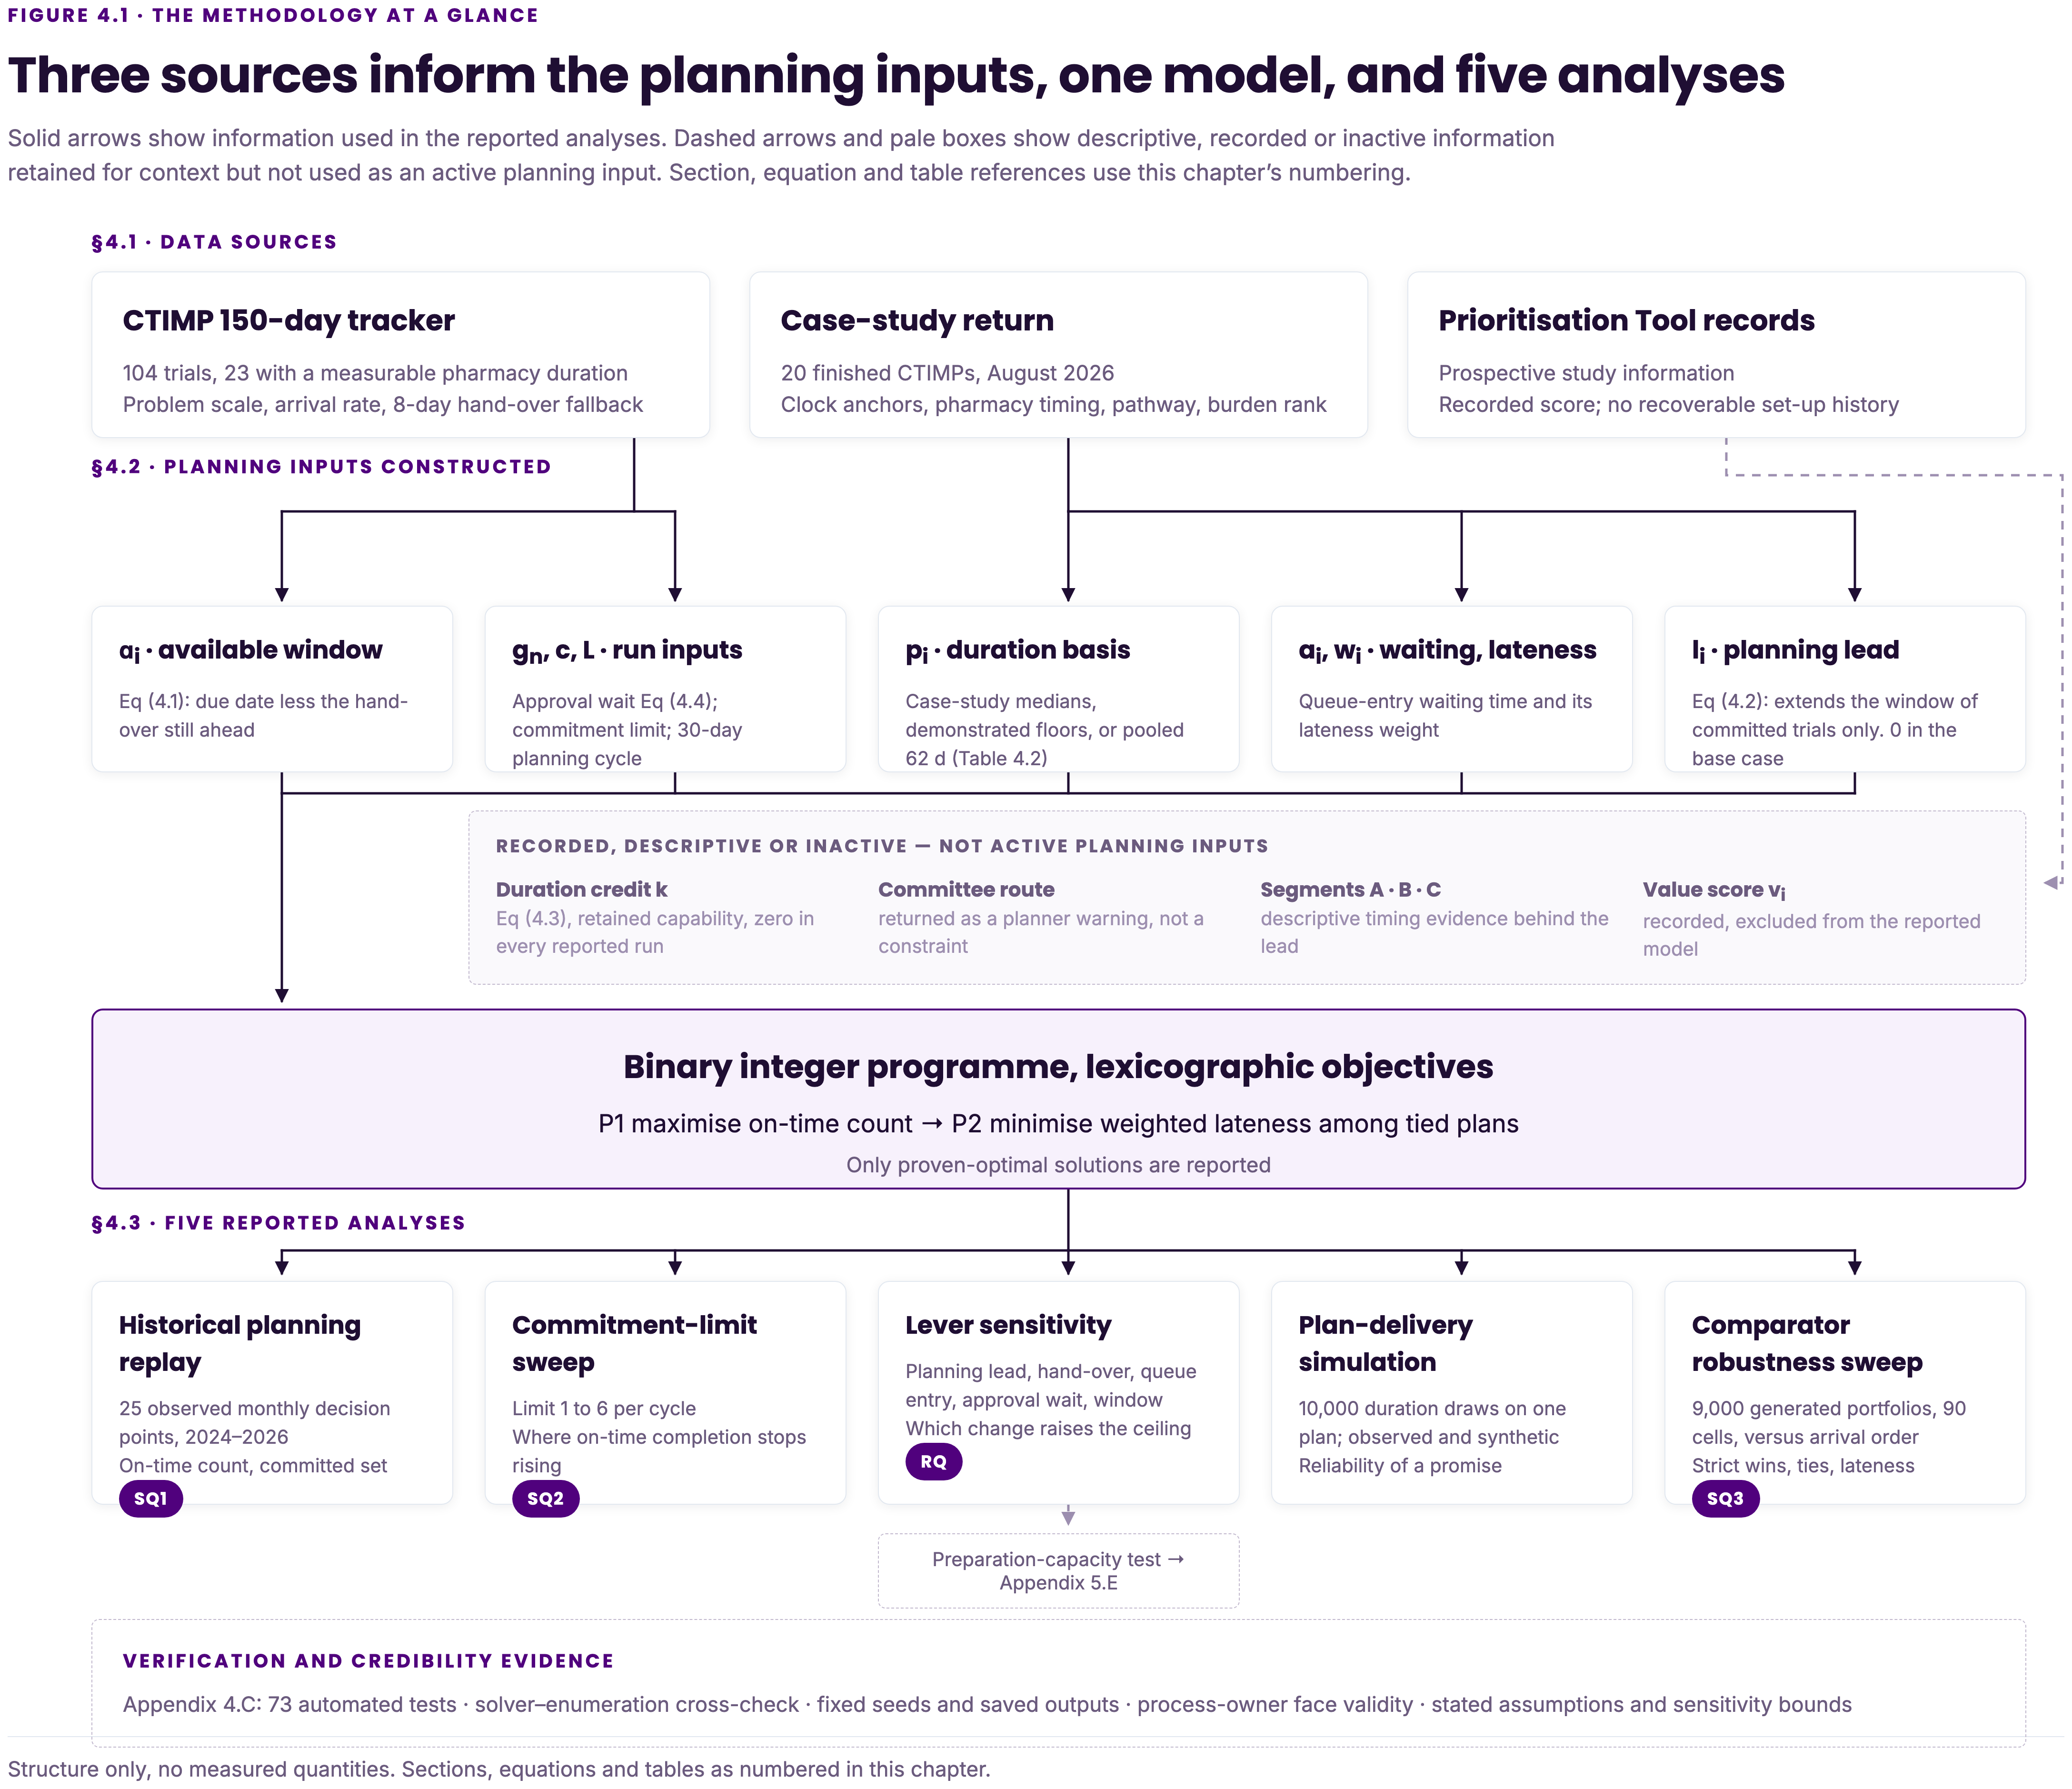
\includegraphics[width=\textwidth]{fig4_1_methodology_map.png}
  \caption{From operational records to research-question evidence}
  \label{fig:datasources}
\end{figure}

\section{Constructing the planning inputs}
\label{sec:parameters}

Four quantities decide a plan. Appendix 4.J tabulates every parameter, its source, and the two quantities deliberately excluded.

\subsection{Days available, which is not days remaining}
\label{sec:available}

A trial's available time is the period from the point at which pharmacy can begin work to its due date:

\begin{equation}
  \alpha_i = due_i - \max(\text{today}, \; \text{queue entry}_i)
  \label{eq:available}
\end{equation}

The calculation subtracts hand-over delay that is still ahead of the trial, but not delay already served. This distinguishes the nominal 60-day deadline from the time pharmacy can actually use; Figure~\ref{fig:segments} illustrates the distinction.

\begin{figure}[htbp]
  \centering
  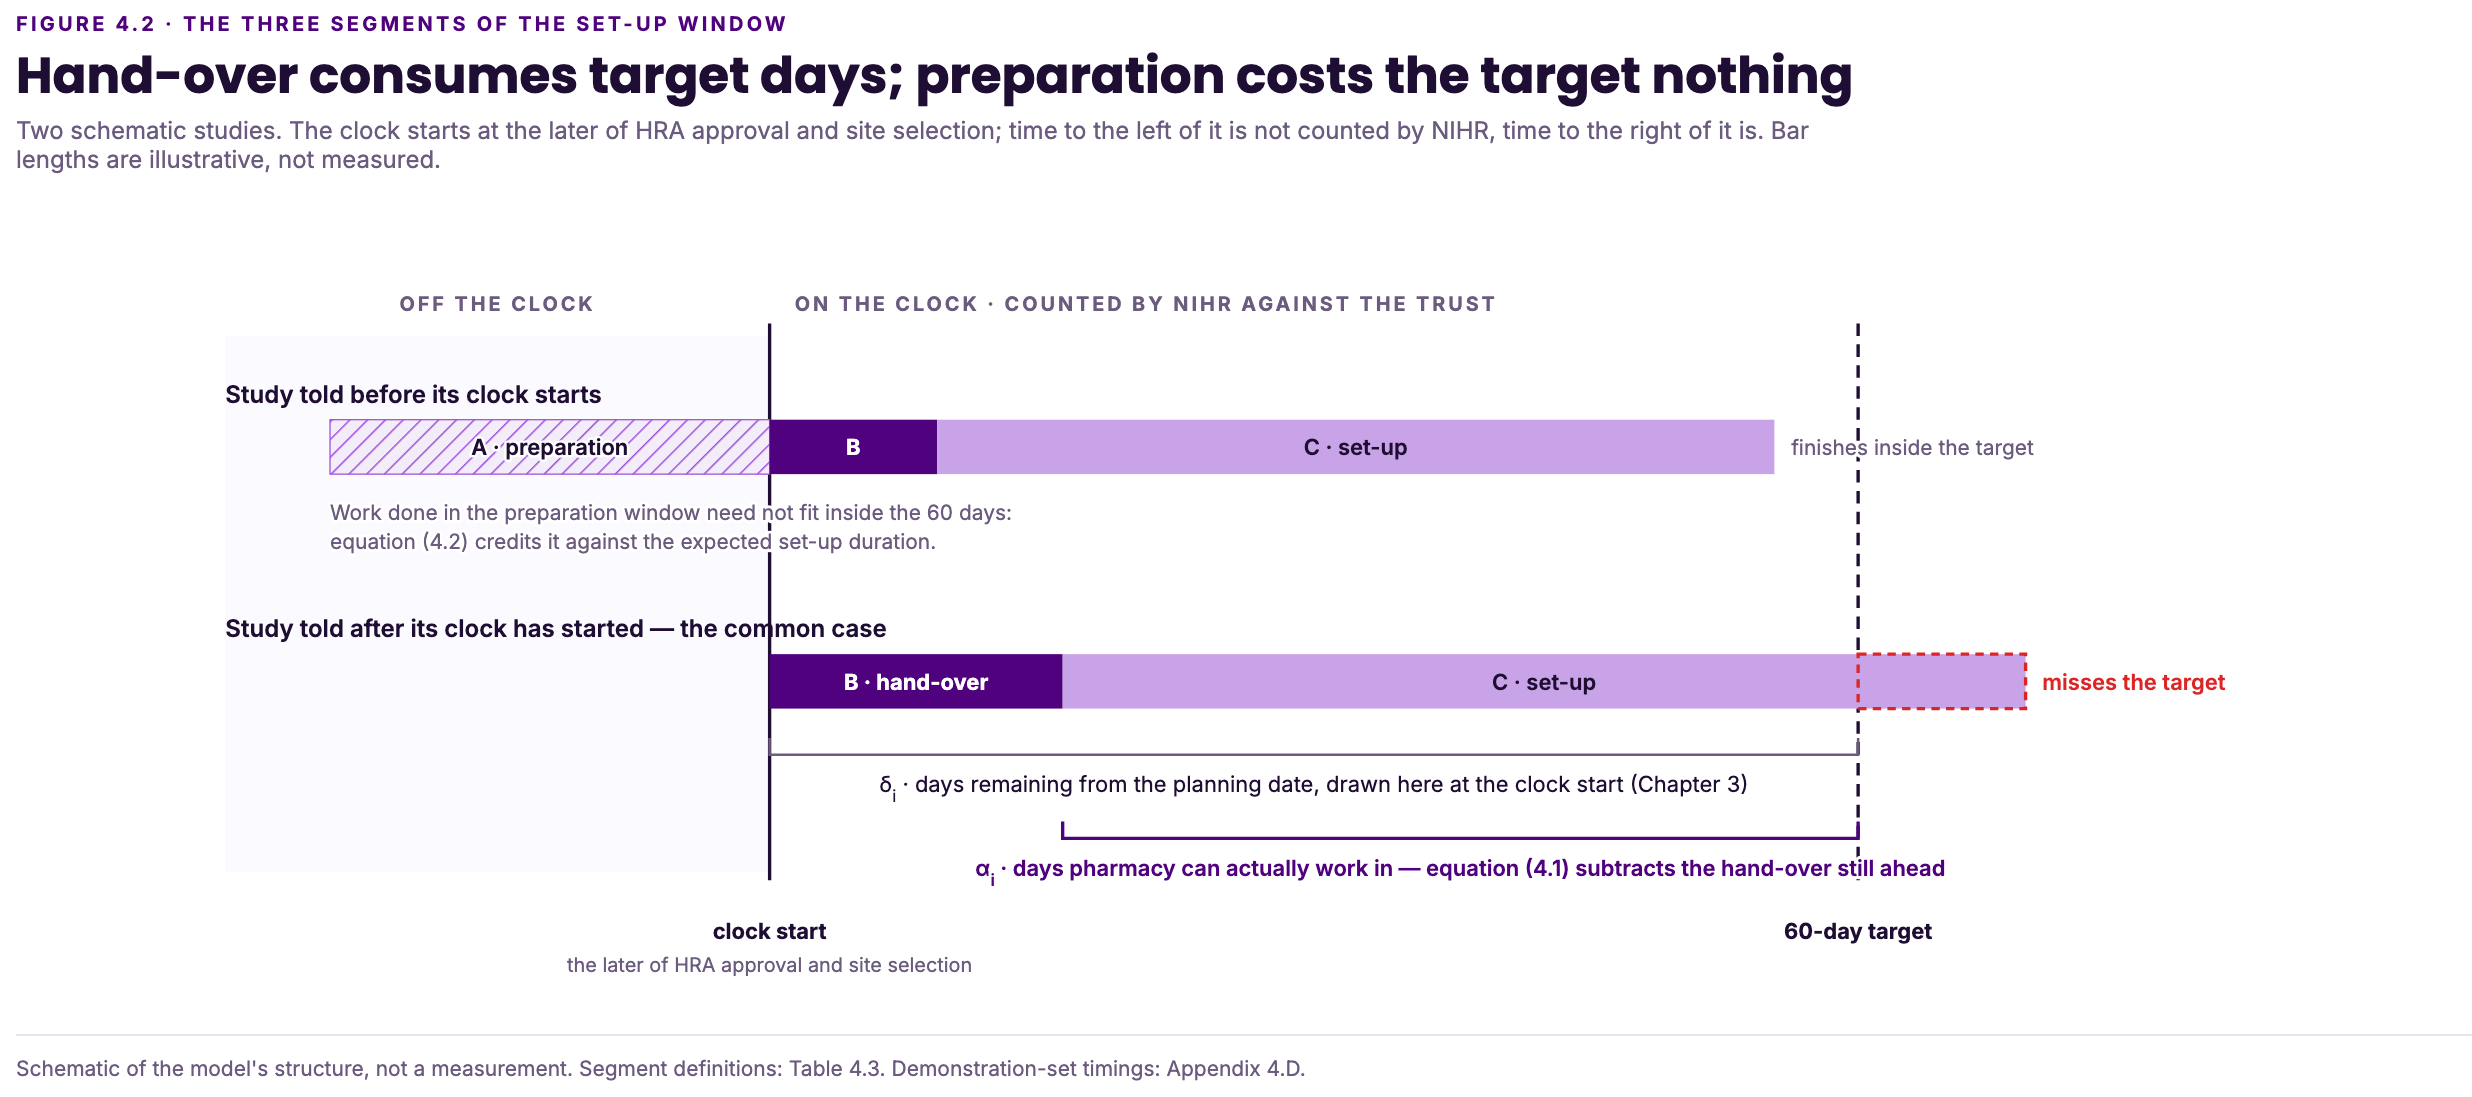
\includegraphics[width=\textwidth]{fig4_2_segment_schematic.png}
  \caption{Hand-over consumes target days; preparation costs the target nothing \emph{Note.} A schematic of the model's structure, not a measurement. Measured distributions are in Appendix 4.D.}
  \label{fig:segments}
\end{figure}

\subsection{Set-up duration, treated as uncertain}
\label{sec:casestudies}

The duration basis differs by analysis. Current-performance regimes use elapsed case-study durations, whereas the demonstrated planning floors are derived from recorded work intervals. All duration measures end at pharmacy green light, but their start events differ; Appendix 4.H defines each interval and Appendix 4.B considers the resulting overlap with approval delay. Across the 19 usable work intervals, the median was 79 days, with a range of 23 to 262 days; five fitted within the 60-day target.

\begin{table}[htbp]
  \centering
  \caption{The five duration regimes}
  \label{tab:regimes}
  \begin{tabularx}{\textwidth}{@{}lLL@{}}
    \toprule
    \textbf{Regime} & \textbf{What it represents} & \textbf{Where used} \\
    \midrule
    0.8 times the case-study medians & Current performance 20\% faster & Appendix 5.A \\
    \addlinespace
    1.0 times the case-study medians & Current performance & Appendix 5.A \\
    \addlinespace
    1.2 times the case-study medians & Current performance 20\% slower & Appendix 5.A \\
    \addlinespace
    The demonstrated work floors & Routine 50; Prescription-only 30; Aseptic-only 72; Both 60 days. A 63-day overlay applies only to high-burden studies on the Both pathway & §Section~\ref{sec:realqueues} to 5.6, Appendix 5.A \\
    \addlinespace
    The pooled first-quartile figure of 62 days & One achievable benchmark across pathways & Appendix 5.A \\
    \bottomrule
  \end{tabularx}
\end{table}

High burden means a rank of 5 or 6 on the scale pharmacy returned; Appendix 4.H distinguishes the burden-band minima, the pathway floors and the 63-day overlay, and Appendix 4.F explains why that rank is the one used.

The floors are demonstrated-achievable standards rather than forecasts or raw minima; Appendix 4.H derives and audits them. Results computed on them describe an optimistic operating condition rather than an expected one.

\subsection{Preparation and approval}
\label{sec:preparation}

Preparation does not shorten the total work a trial requires; it moves part of that work outside the target window. The case studies suggest that earlier starts change how much work falls within the target window rather than the observed work duration itself: work intervals did not differ detectably between early and late starters, whereas on-time outcomes did (Appendix 4.I).

The reported preparation analysis represents an earlier planning lead, which for committed trials increases the time available before the 60-day deadline. It is interpreted operationally as work that can begin before the target clock starts, rather than as evidence that underlying set-up duration is shorter. Writing $\ell_i$ for the lead assigned to a committed trial:

\begin{equation}
  \alpha_i^{\text{lead}} = \alpha_i + \ell_i
  \label{eq:lead}
\end{equation}

The lead is granted only to committed trials and is zero in the base case; Appendix 4.J.3 gives the implementation.

The base analysis does not charge pre-window preparation against the cycle commitment limit. This isolates the time benefit of earlier preparation from its operational resource cost; Appendix 5.E tests the sensitivity of that simplification by reducing the concurrent capacity available to the plan.

The implementation retains a separate duration-credit capability, but it is inactive in every reported analysis and produces no Chapter 5 result; its specification and verification are retained in Appendix 4.J.4 and Appendix 4.C, Tests 24 to 35.

Final approval is a shared, load-dependent queue. The wait $g_n$ uses the Pollaczek-Khinchine formula for a single server, exact when its assumptions hold and needing only the mean and variability of approval time, not its shape, which this study cannot observe:

\begin{equation}
  g_n = \frac{\rho}{1-\rho} \cdot \frac{1+\kappa^2}{2} \cdot s, \qquad \rho = \min\left(0.95,\; \frac{n\,s}{A}\right)
  \label{eq:pk}
\end{equation}

Approval time is unobserved and is therefore treated as a sensitivity parameter; Appendix 4.B records the queueing assumptions, the utilisation and variability values, and the overlap analysis.

\section{Experimental design}
\label{sec:experiments}

Every run builds a plan by the process in Figure~\ref{fig:solution}, differing only in what it varies before that process starts and records after it ends. The model maximises on-time completions first and then minimises weighted lateness among tied plans. For Section~\ref{sec:tradeoff}, the model also reports the least-late plan at each achievable on-time count to display the trade-off; these are count-constrained comparisons, not alternative lexicographic optima. Appendix 4.J provides the formulation and solver settings.

\begin{figure}[htbp]
  \centering
  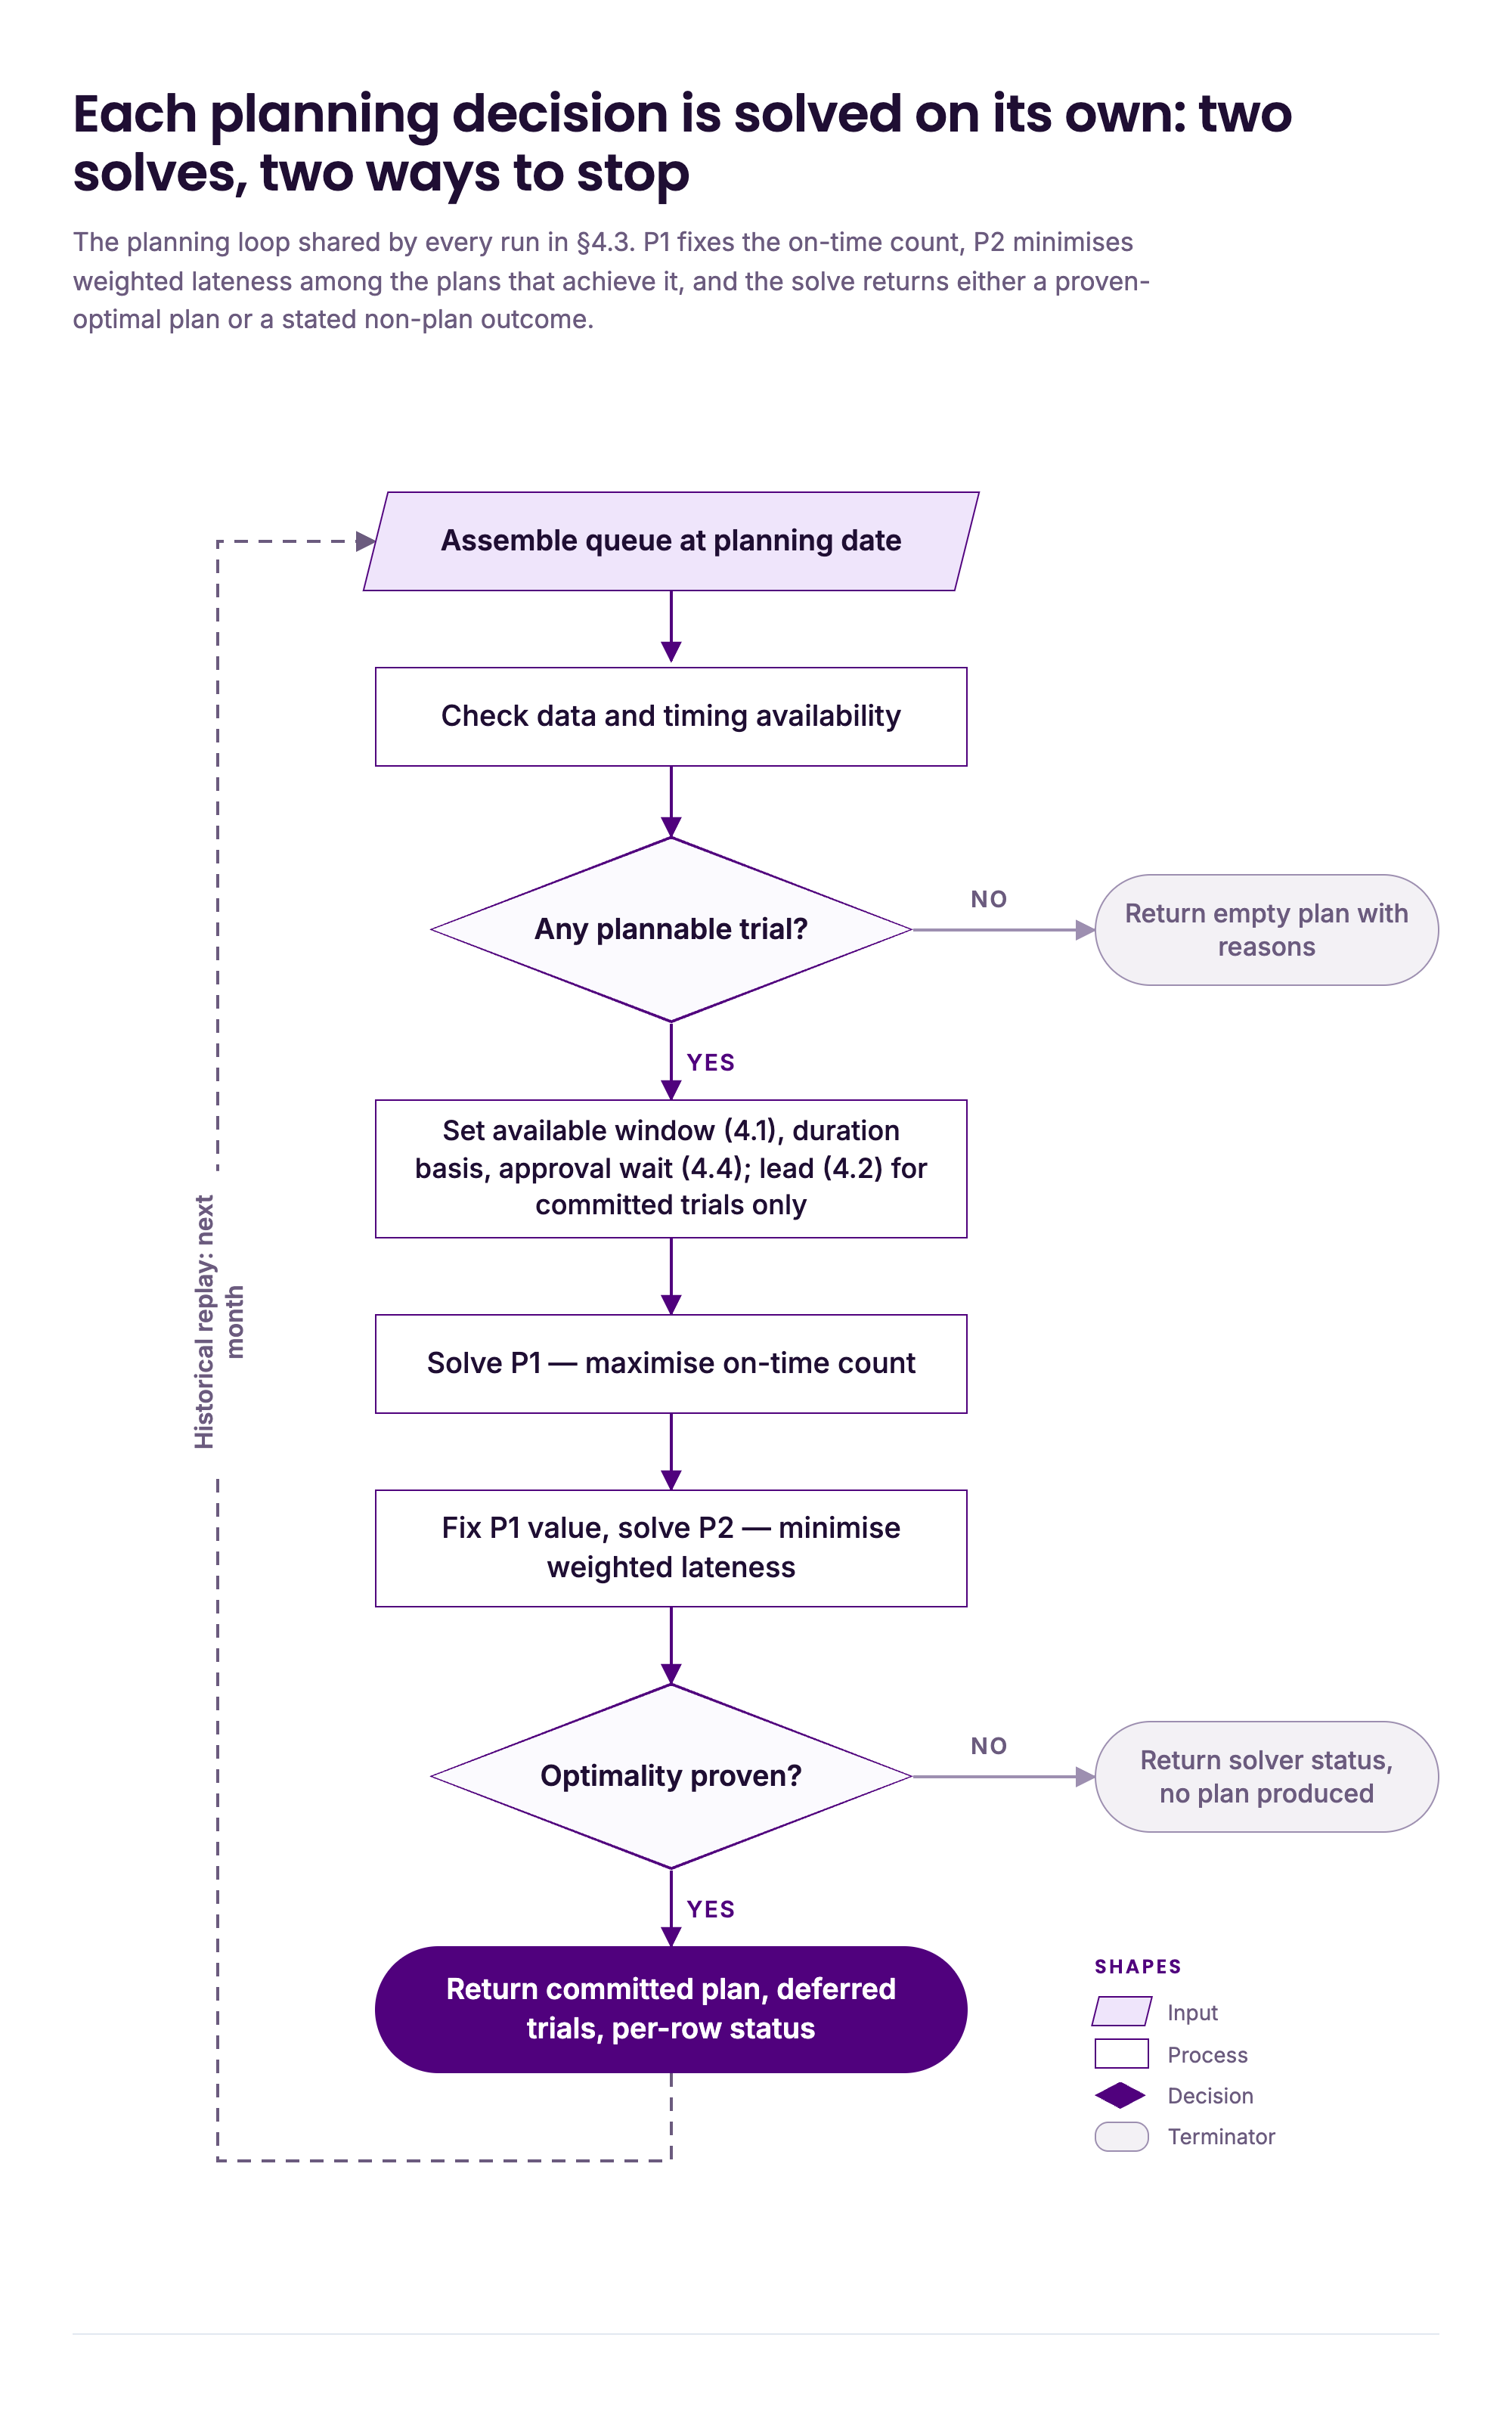
\includegraphics[width=\textwidth]{fig4_3_solution_construction.png}
  \caption{Solution construction process \emph{Note.} The dashed return arrow applies to the historical replay only: each month is solved independently and no slot is held open for a later one.}
  \label{fig:solution}
\end{figure}

\begin{table}[htbp]
  \centering
  \caption{Analysis-to-question map}
  \label{tab:analyses}
  \begin{tabularx}{\textwidth}{@{}lLLLL@{}}
    \toprule
    \textbf{Analysis} & \textbf{Data basis} & \textbf{What varies} & \textbf{What it measures} & \textbf{Question} \\
    \midrule
    Historical planning replay & Observed queues & 25 monthly decision points, 2024 to 2026 & On-time trials, committed set & SQ1 \\
    \addlinespace
    Commitment-limit sweep & Observed queues & Commitments per cycle, 1 to 6 & Whether raising the commitment limit changes on-time completion or weighted lateness & SQ2 \\
    \addlinespace
    Lever sensitivity & Observed queues & Preparation, hand-over, queue entry, approval, target window & Which change raises the ceiling & RQ, SQ2 \\
    \addlinespace
    Plan-delivery simulation & Observed and synthetic queues & 10,000 duration draws on one plan & Reliability of a promised outcome & RQ \\
    \addlinespace
    Comparator robustness sweep & Generated portfolios & 9,000 portfolios, 90 scenario cells & Strict wins over arrival order, and their cost & SQ3 \\
    \addlinespace
    Targeted-preparation comparison & Observed queues & Lead to high-burden committed trials only, against all committed trials & On-time coverage and the early-notification days required & Appendix 5.B \\
    \addlinespace
    Preparation-capacity test & Observed queues & Preparation lead against reduced capacity & Whether the preparation finding survives & Appendix 5.E \\
    \bottomrule
  \end{tabularx}
\end{table}

Nineteen case studies enter the replay, being those with both clock anchors; BALLOON has no site-selected date and BRISOTE no recorded start. Appendix 4.J holds the run settings, of which one hands-on day per approval is the only input in Chapter 5 not measured.

Two simulations are reported separately. The plan-delivery simulation tests the reliability of a selected plan under duration uncertainty, whereas the robustness sweep tests whether the selection rule outperforms arrival order across generated portfolios. Appendix 4.J specifies their distributions, settings and reporting rules.

\subsection{The comparator and the robustness sweep}
\label{sec:comparison}

\textbf{The comparator is arrival order} (Section~\ref{sec:inpractice}): it commits the longest-waiting eligible trials up to the same commitment limit as the model. Both plans run through Figure~\ref{fig:solution} under identical windows, duration assumptions and approval waits, so any difference arises from the selected set alone. Because practice may informally expedite some studies, the comparator result is an upper bound on the model's advantage over routine practice.

The sweep generates portfolios that vary arrival timing, pathway composition and duration regime, and reports the count in which the model places strictly more trials inside the window, with ties and the weighted-lateness difference beside it. Appendix 4.J.6.1 specifies the design and states why ties are read at cell level rather than pooled. \textbf{Table 5.A.2 summarises the sweep by duration regime and is the principal test of SQ3}; Appendix 5.A holds the grid.

\section{Credibility, assumptions and boundaries}
\label{sec:verification}

\textbf{Verification, reproducibility and face validity.} Automated tests verify input construction, optimisation logic, simulation behaviour and agreement between enumerated and solver solutions, with the full inventory in Appendix 4.C. All simulation runs use fixed seeds and save dated outputs, so Chapter 5 figures can be regenerated exactly. R\&I and pharmacy reviewed the process representation and input definitions, which constitutes face validity from process owners rather than independent validation.

\textbf{A known overlap, bounded rather than removed.} Each planning duration ends at the pharmacy green light, which is the approving signature, so it already includes part of the wait that equation~(\ref{eq:pk}) adds separately. That component is dated in no system and cannot be separated, so the overlap is retained as a bounded conservative approximation rather than an empirically identified separation of work and approval delay; Appendix 4.B gives the assumption audit and the sensitivity result.

\textbf{What the evidence cannot establish.} Three limits bound every result. Set-up start dates are estimates, so the durations of Section~\ref{sec:casestudies} carry recall error the data cannot quantify. Hands-on approval time is unmeasured, so the checks above verify the implementation and not the formulation behind equation~(\ref{eq:pk}); testing that needs a separate model of the approval-signature queue, recorded as future work in Chapter 6. And the generated data of Section~\ref{sec:experiments} answer questions the observed queues cannot, but do not evidence the trust's own portfolio. All three are handled by stated assumption, sensitivity analysis and simulation rather than presented as observed fact.

---

